% =====================================================================
% Abschnitt 4: Durchführung der Experimente und Ergebnisse
% Generiert auf Basis der realen Notebook-Ausführungen und Metrik-Dateien
% unter thesis_experiments/results/ (TF1-TF4) sowie der finalen
% Gesamtpipeline (finale_bereinigung_summary.json).
% Bilder liegen unter thesis_experiments/images/
% =====================================================================

\section{Durchführung der Experimente und Ergebnisse}

Für jede der vier Teilforschungsfragen (TF1 bis TF4) wurden drei methodische
Ansätze auf identischen Trainings-/Testaufteilungen (\texttt{split} = \texttt{train}
bzw. \texttt{test}) desselben Benchmarks evaluiert: ein klassischer, regelbasierter
bzw. unüberwachter Basisansatz, ein moderner Non-LLM-Ansatz aus dem Bereich des
maschinellen Lernens sowie Anthropics Sprachmodell Claude (\texttt{claude-sonnet-5})
über die offizielle API. Alle in diesem Abschnitt berichteten Zahlenwerte stammen
unmittelbar aus den tatsächlichen Ausführungsprotokollen der zugehörigen Jupyter-Notebooks
(\texttt{results/*\_metrics.json}, \texttt{results/*\_predictions.csv}) und wurden nicht
nachträglich verändert oder geglättet.

% ---------------------------------------------------------------------
\subsection{Experiment 1: Erkennung und Entfernung von Duplikaten (TF1)}
\label{sec:experiment-tf1}

Die Duplikaterkennung wurde auf einem Benchmark von 148 Test-Paaren (davon 37
tatsächliche Duplikate und 111 Nicht-Duplikate) evaluiert. Tabelle
\ref{tab:tf1-ergebnisse} fasst die Ergebnisse der drei Methoden zusammen.

\begin{table}[htbp]
\centering
\caption{Ergebnisse Experiment 1 - Duplikaterkennung (TF1), $n_{\text{test}} = 148$ Paare}
\label{tab:tf1-ergebnisse}
\begin{tabular}{lccccc}
\toprule
\rowcolor{headerblue}
\textbf{Methode} & \textbf{Precision} & \textbf{Recall} & \textbf{F1-Score} & \textbf{FP} & \textbf{FN} \\
\midrule
\rowcolor{lightgray}
Exact-Match + RapidFuzz (Baseline) & 0{,}949 & 1{,}000 & 0{,}974 & 2 & 0 \\
Splink (Fellegi-Sunter, EM-Algorithmus) & 1{,}000 & 0{,}973 & 0{,}986 & 0 & 1 \\
\rowcolor{lightgray}
Claude LLM (\texttt{claude-sonnet-5}) & 1{,}000 & 0{,}973 & 0{,}986 & 0 & 1 \\
\bottomrule
\end{tabular}
\end{table}

Abbildung \ref{fig:tf1-methodenvergleich} stellt die drei Methoden grafisch
gegenüber. Splink und das LLM erzielen mit $F1 = 0{,}986$ exakt denselben
Score, jedoch über unterschiedliche Fehlerprofile: Splink benötigte für Training
und Vorhersage zusammen ca. 38,6 Sekunden ohne API-Kosten, während das LLM
für dieselbe Aufgabe 383,7 Sekunden (rund 6,4 Minuten) sowie 119.432
Input- und 14.811 Output-Tokens (geschätzte Kosten: 0,387 USD) benötigte - bei
identischer Ergebnisqualität also ein Faktor von etwa 10 in der Laufzeit
zugunsten von Splink.

\begin{figure}[htbp]
\centering
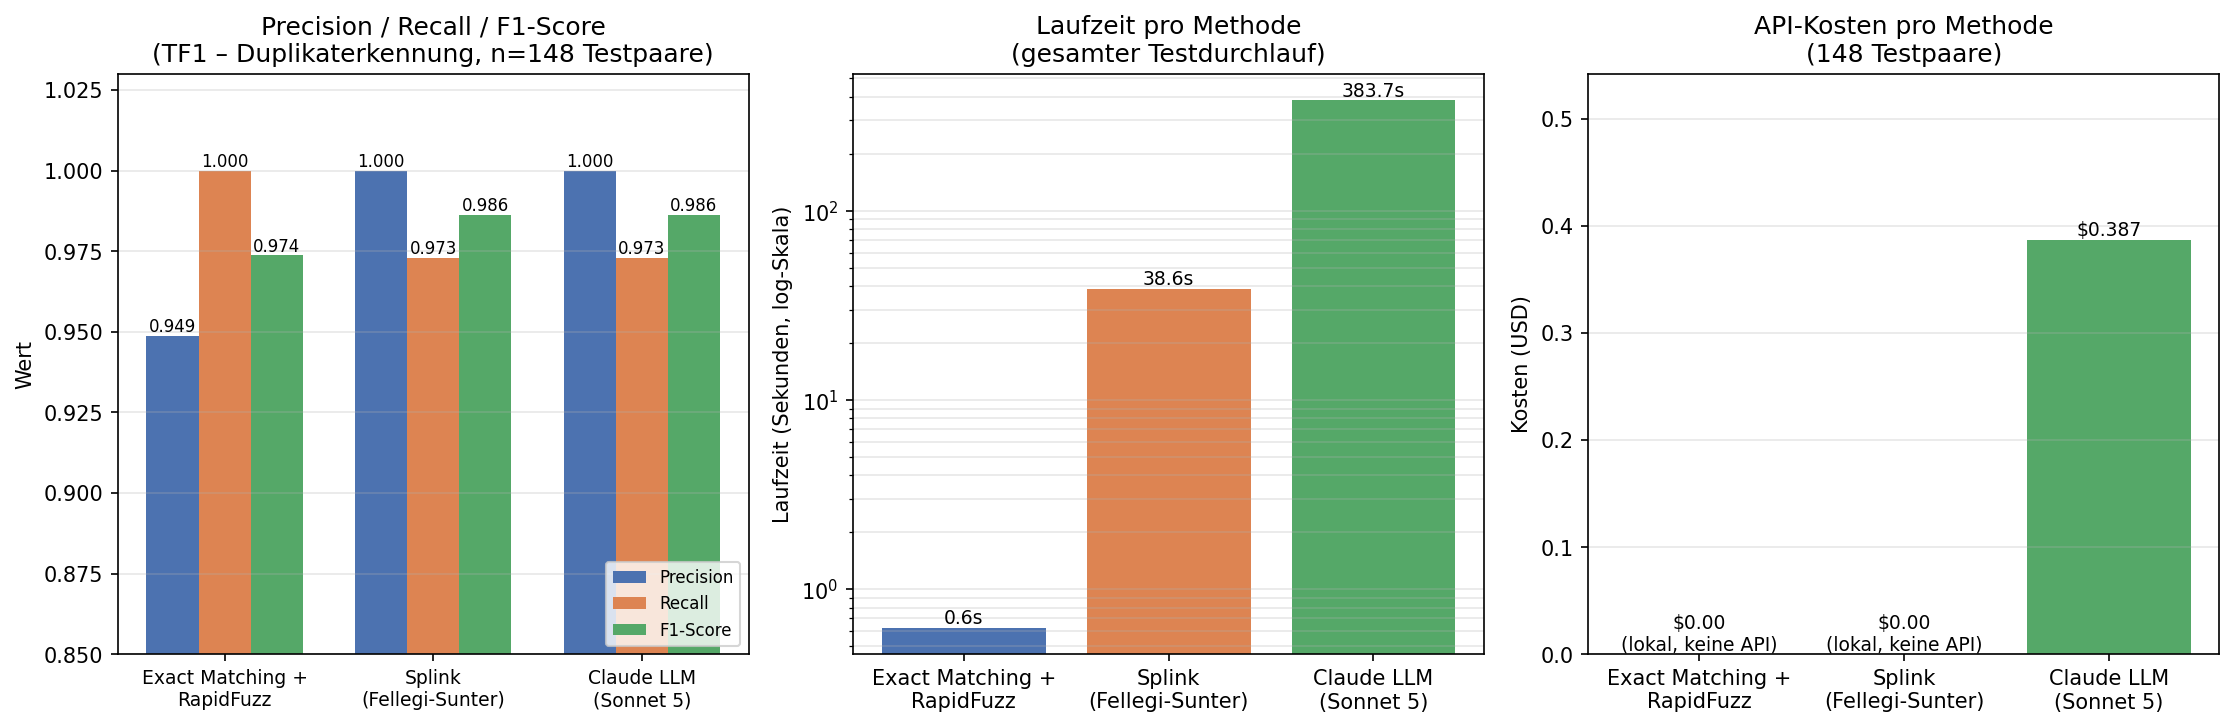
\includegraphics[width=0.85\textwidth]{images/tf1_methodenvergleich.png}
\caption{Methodenvergleich TF1 - Precision, Recall und F1-Score im direkten Vergleich}
\label{fig:tf1-methodenvergleich}
\end{figure}

\subsubsection{Baseline: Exact-Match + RapidFuzz}

Die Baseline kombiniert einen exakten URL-Abgleich mit einem
Zeichenketten-Ähnlichkeitsmaß (RapidFuzz) auf den Thread-Titeln und einem
Schwellenwert von 51 (bei einer Ähnlichkeitsskala von 0 bis 100). Sie erreicht
mit $F1 = 0{,}974$ bereits ein bemerkenswert hohes Niveau, produziert jedoch
zwei falsch-positive Klassifikationen. Beide Fehlerfälle sind aufschlussreich,
da sie eine strukturelle Schwäche rein zeichenkettenbasierter Verfahren
offenlegen: Die Titel \enquote{TrekPow G39 1200A \$67.99 57\% off} und
\enquote{Rhino 16000lbs ramp \$69.99 + FS} beschreiben zwei völlig
unterschiedliche Produkte (ein Batterie-Ladegerät und eine Auffahrrampe),
teilen sich jedoch zufällig ein sehr ähnliches Preis-/Rabatt-Zahlenformat
(\enquote{\$xx.99}, Prozentangabe), wodurch die Ähnlichkeitsberechnung einen
Score von 52{,}6 - knapp über dem Schwellenwert - ergibt. Ein zweites,
ähnlich gelagertes Paar betraf ein Kreditkarten-Angebot (\enquote{Collect \$100
CT Money on \$250+ spend at Canadian Tire Auto Service Centre}) und ein
American-Express-Angebot, die über wiederkehrende Dollar-Beträge im Titeltext
fälschlicherweise als Duplikat markiert wurden. Die Baseline erkennt somit
\emph{Zahlenmuster}, nicht \emph{semantische Produktidentität}.

\subsubsection{Moderner Non-LLM-Ansatz: Splink (Fellegi-Sunter-Modell)}

Splink implementiert ein probabilistisches Record-Linkage-Verfahren nach
Fellegi und Sunter, bei dem paarweise Übereinstimmungsgewichte pro Merkmal
(u.\,a. Titel-Ähnlichkeit, URL, Kategorie) über einen Expectation-Maximization-Algorithmus
gelernt und zu einer Gesamt-Match-Wahrscheinlichkeit kombiniert werden. Dieses
Modell erreicht eine perfekte Precision von 1{,}0 - es produziert keinen
einzigen falsch-positiven Treffer -, verpasst jedoch ein echtes Duplikat: Die
beiden Einträge \enquote{Kawasaki 1.2 GPM @ 1,650 PSI Electric Pressure
Washer} und \enquote{Kawasaki 1650 PSI Pressure Washer \$139} beschreiben
dasselbe Produkt, unterscheiden sich jedoch so stark in Formulierung,
Zeichensetzung und enthaltenen Zusatzinformationen (Marke vs. Modellnummer vs.
Preis im Titel), dass Splink ihnen nur eine Match-Wahrscheinlichkeit von
$0{,}004$ zuweist - weit unter dem gewählten Schwellenwert von $0{,}01$. Dieser
Einzelfall bestätigt eine bereits in Abschnitt 3.3 dokumentierte methodische
Erkenntnis dieser Arbeit: Da Splink allein gelegentlich zu unspezifisch bzw.
in Grenzfällen zu konservativ urteilt, wurde für die finale Pipeline (siehe
Abschnitt \ref{sec:finale-anwendung}) eine zusätzliche regelbasierte
Titel-Plausibilitätsprüfung ergänzt.

\subsubsection{Claude LLM}

Das Sprachmodell erhielt die vollständigen Metadaten beider Kandidaten eines
Paares (Titel, Kategorie, Quelle, Preis) im Prompt und wurde gebeten, eine
begründete Ja/Nein-Entscheidung zu treffen. Mit $F1 = 0{,}986$ erzielt es exakt
denselben Score wie Splink. Bemerkenswert ist jedoch die Natur des einzigen
Fehlers: Das vom LLM tatsächlich falsch beurteilte Paar - \enquote{Body Glove
Porter Inflatable Kayak \$599.99} vs. \enquote{Body Glove Porter Inflatale
Kayak \$599.99} (man beachte den Tippfehler \enquote{Inflatale} statt
\enquote{Inflatable}) - ist ein für ein Sprachmodell inhaltlich triviales
Duplikat. Der protokollierte Fehler ist im Rohprotokoll explizit als
\texttt{[FEHLER/FALLBACK - kein gültiges LLM-Ergebnis]} vermerkt, das heißt,
er ist auf eine technische Antwort-Fallback-Situation (kein aus der
API-Antwort parsbares Urteil) zurückzuführen und nicht auf eine inhaltliche
Fehleinschätzung des Modells. Inhaltlich hätte das LLM diesen Fall also
voraussichtlich korrekt gelöst.

\subsubsection*{Zwischenfazit TF1}

Alle drei Methoden liegen in der Gesamtgüte bemerkenswert nah beieinander
($F1$ zwischen 0{,}974 und 0{,}986). Für die konkrete Aufgabe der
Duplikaterkennung auf strukturierten Kleinanzeigen-/Angebotsdaten bietet der
moderne Non-LLM-Ansatz (Splink) bei identischer Ergebnisqualität wie das LLM
einen klaren Laufzeit- und Kostenvorteil (siehe Abschnitt
\ref{sec:laufzeit-kosten}), während das LLM seine Stärke vor allem in der
Interpretierbarkeit der Einzelentscheidungen (textuelle Begründung je Paar)
ausspielt, ohne diese hier in eine höhere Endgenauigkeit übersetzen zu können.

% ---------------------------------------------------------------------
\subsection{Experiment 2: Behandlung fehlender Werte (TF2)}
\label{sec:experiment-tf2}

Für TF2 wurden zwei Zielattribute mit künstlich eingefügten fehlenden Werten
betrachtet: das numerische Attribut \texttt{price} ($n_{\text{test}} = 164$)
sowie das kategoriale Attribut \texttt{parent\_category} ($n_{\text{test}} =
125$). Tabelle \ref{tab:tf2-ergebnisse} zeigt die Ergebnisse.

\begin{table}[htbp]
\centering
\caption{Ergebnisse Experiment 2 - Fehlende Werte (TF2)}
\label{tab:tf2-ergebnisse}
\begin{tabular}{lcccc}
\toprule
\rowcolor{headerblue}
\textbf{Methode} & \textbf{price MAE} & \textbf{price RMSE} & \textbf{parent\_cat. Acc.} & \textbf{parent\_cat. Macro-F1} \\
\midrule
\rowcolor{lightgray}
Median/Modus (Baseline) & 189{,}40 & 362{,}30 & 0{,}912 & 0{,}858 \\
Random Forest n.\ MissForest-Prinzip & 176{,}34 & 294{,}68 & 0{,}856 & 0{,}827 \\
\rowcolor{lightgray}
Claude LLM & \textbf{154{,}30} & \textbf{292{,}40} & 0{,}888 & 0{,}853 \\
\bottomrule
\end{tabular}
\end{table}

\begin{figure}[htbp]
\centering
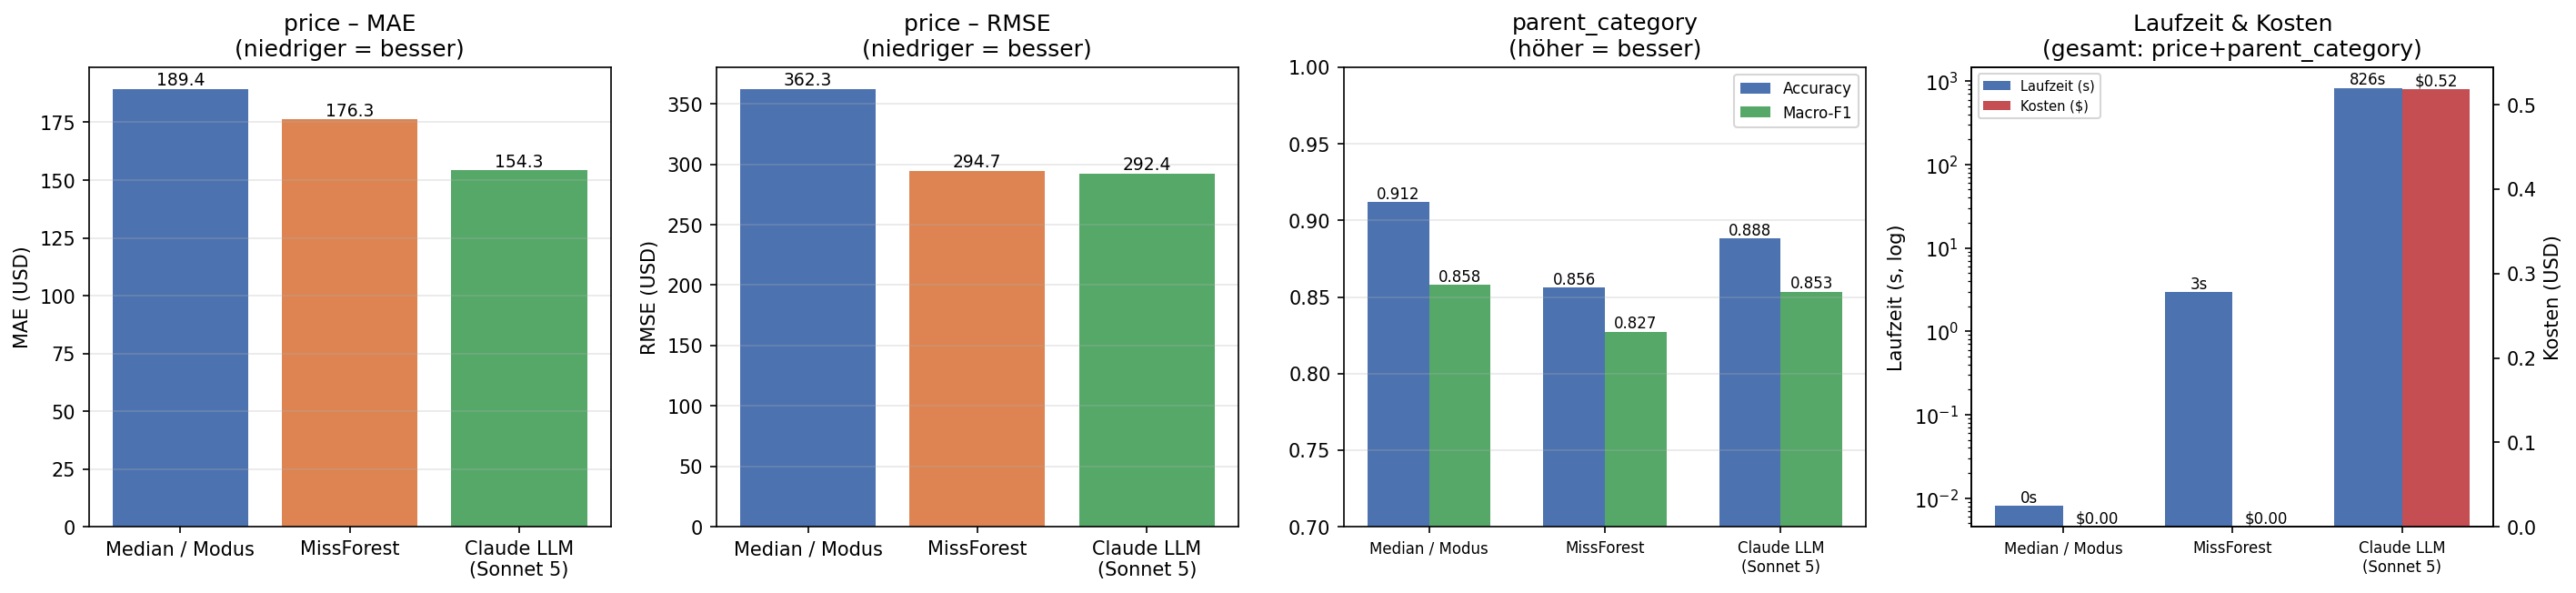
\includegraphics[width=0.85\textwidth]{images/tf2_methodenvergleich.png}
\caption{Methodenvergleich TF2 - Fehlerkennzahlen für \texttt{price} und \texttt{parent\_category}}
\label{fig:tf2-methodenvergleich}
\end{figure}

\subsubsection{Von HyperImpute zu Random-Forest-Imputation nach dem MissForest-Prinzip}

Wie in Abschnitt 3.2.2 methodisch erläutert, konnte die ursprünglich
vorgesehene AutoML-Bibliothek HyperImpute aufgrund eines reproduzierbaren
Kompatibilitätsproblems mit den installierten scikit-learn-/pydantic-Versionen
nicht produktiv eingesetzt werden. Als Ersatz wurde direkt das dem
MissForest-Verfahren (Stekhoven \& Bühlmann, 2012)\autocite{stekhoven2012missforest}
zugrunde liegende Random-Forest-Prinzip implementiert - mit der methodisch
wichtigen Einschränkung, dass es sich hierbei um separate, einmalig trainierte
\texttt{RandomForestRegressor}-/\texttt{RandomForestClassifier}-Modelle je
Zielattribut handelt und nicht um eine vollständige iterative
MissForest-Implementierung (siehe Abschnitt 3.2.2 für die vollständige
Herleitung dieser Einschränkung).

\subsubsection{Quantitative Ergebnisse und Trade-off zwischen den Methoden}

Bei der numerischen Vorhersage von \texttt{price} zeigt sich eine klare
Rangfolge: Das LLM erzielt mit MAE $= 154{,}30$ den niedrigsten Fehler, gefolgt
von der Random-Forest-Imputation (MAE $= 176{,}34$) und zuletzt der
Median-Baseline (MAE $= 189{,}40$). Interessanterweise kehrt sich diese
Rangfolge beim kategorialen Zielattribut \texttt{parent\_category} teilweise
um: Hier erzielt die einfache Modus-Baseline (\enquote{häufigste
\texttt{parent\_category} je \texttt{thread\_category}}) mit einer Genauigkeit
von 0{,}912 das beste Ergebnis alter drei Methoden, noch vor dem LLM (0{,}888)
und der Random-Forest-Klassifikation (0{,}856). Dies lässt sich dadurch
erklären, dass die Zuordnung \texttt{thread\_category} $\rightarrow$
\texttt{parent\_category} im vorliegenden Datensatz größtenteils sehr
konsistent und nahezu deterministisch ist (siehe auch die Diskussion der
Dictionary-Methode in Abschnitt \ref{sec:experiment-tf4}), wodurch eine simple
Nachschlagetabelle bereits ein sehr starker Prädiktor ist und die
zusätzliche Modellkomplexität von Random Forest bzw. LLM hier keinen Mehrwert,
sondern teilweise sogar zusätzliches Rauschen einbringt.

Ein konkretes Fallbeispiel verdeutlicht die Unterschiede im Umgang mit echten
Ausreißern: Für Zeile 156 (wahrer Preis 1029{,}00 USD, vermutlich ein
hochpreisiges Elektronikprodukt) sagt die Median-Baseline lediglich 50{,}30
USD voraus (absoluter Fehler 978{,}70), die Random-Forest-Imputation 96{,}43
USD (Fehler 932{,}57) und das LLM 599{,}99 USD (Fehler 429{,}01) - das LLM
liegt damit zwar ebenfalls deutlich daneben, jedoch um ein Vielfaches näher am
wahren Wert, vermutlich weil es aus den Zusatzmerkmalen (\texttt{thread\_category},
\texttt{source}) einen plausibleren Preisrahmen ableiten kann. Umgekehrt zeigt
Zeile 892 (wahrer Preis lediglich 1{,}00 USD, vermutlich ein
Gratis-/Symbolpreis-Angebot) das gegenteilige Bild: Hier liegt das LLM mit
4{,}99 USD (Fehler 3{,}99) am nächsten am wahren Wert, während die
Random-Forest-Imputation mit 88{,}86 USD (Fehler 87{,}86) deutlich stärker
danebenliegt als selbst die Median-Baseline (9{,}995 USD, Fehler 8{,}995) -
ein Hinweis darauf, dass Random-Forest-Modelle bei stark linksschiefen
Preisverteilungen mit vereinzelten Nahe-Null-Werten dazu neigen, in Richtung
des Ensemble-Mittelwerts zu regredieren, während das LLM kontextuelle
Hinweise (z.\,B. Formulierungen wie \enquote{gratis} oder \enquote{Cent-Artikel}
im Titel) direkt nutzen kann.

\subsubsection*{Zwischenfazit TF2}

Die Ergebnisse von TF2 zeigen deutlicher als jedes andere Experiment dieser
Arbeit, dass es \emph{keine universell beste Methode} gibt: Für die
numerische Preisvorhersage liefert das LLM die besten Ergebnisse, für die
kategoriale Klassifikation mit stark strukturierter, redundanter
Merkmalsbeziehung schlägt hingegen die triviale Baseline beide komplexeren
Verfahren. Dies unterstreicht die Notwendigkeit, für jede konkrete
Teilaufgabe empirisch zu evaluieren, statt pauschal von einer
Methodenklasse auf ihre Eignung zu schließen.

% ---------------------------------------------------------------------
\subsection{Experiment 3: Behebung von Formatierungsfehlern (TF3)}
\label{sec:experiment-tf3}

TF3 betrachtet drei Zielspalten mit heterogenen Rohformaten: \texttt{price}
($n = 257$), \texttt{saving} ($n = 149$) und Datumsangaben ($n = 885$).
Tabelle \ref{tab:tf3-ergebnisse} zeigt die Exact-Match-Raten (Anteil exakt mit
dem Referenzwert übereinstimmender bereinigter Werte).

\begin{table}[htbp]
\centering
\caption{Ergebnisse Experiment 3 - Formatierungsfehler (TF3), Exact-Match-Raten}
\label{tab:tf3-ergebnisse}
\begin{tabular}{lccc}
\toprule
\rowcolor{headerblue}
\textbf{Methode} & \textbf{price} ($n{=}257$) & \textbf{saving} ($n{=}149$) & \textbf{Datum} ($n{=}885$) \\
\midrule
\rowcolor{lightgray}
Regelbasiert (Regex-Kaskade) & 0{,}992 & 0{,}980 & \textbf{1{,}000} \\
XGBoost-Parser & \textbf{0{,}996} & 0{,}946 & n.\,v.\ \\
\rowcolor{lightgray}
Claude LLM & 0{,}977 & 0{,}946 & \textbf{1{,}000} \\
\bottomrule
\end{tabular}
\end{table}

\begin{figure}[htbp]
\centering
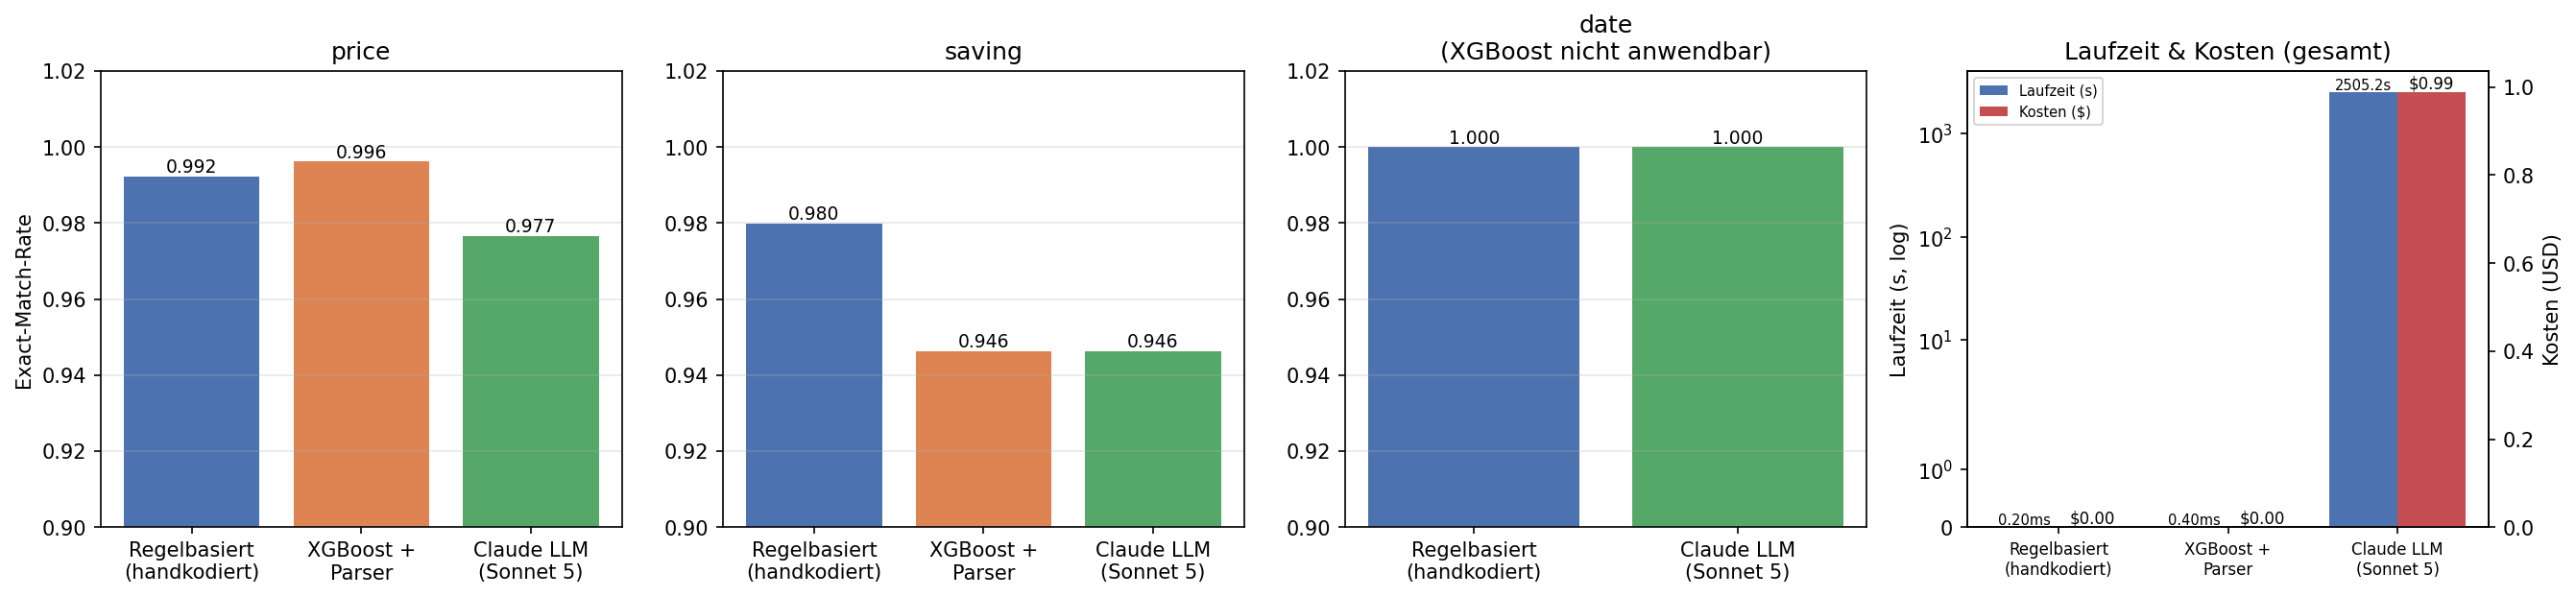
\includegraphics[width=0.85\textwidth]{images/tf3_methodenvergleich.png}
\caption{Methodenvergleich TF3 - Exact-Match-Raten für price, saving und Datum}
\label{fig:tf3-methodenvergleich}
\end{figure}

Bei allen drei Zielspalten liegen die Methoden auf einem durchgehend hohen
Niveau von über 94\,\%, wobei die Datumsnormalisierung von sowohl der
Regex-Kaskade als auch dem LLM fehlerfrei (100\,\%) gelöst wird - ein
Beispiel für einen Rohwert ist \enquote{Jul 16th, 2020 8:29 am}, das beide
Methoden korrekt in das ISO-ähnliche Zielformat
\enquote{2020-07-16 08:29:00} überführen.

\subsubsection{Ein methodisch aufschlussreicher Grenzfall: Wenn die Referenz selbst fehlerhaft ist}

Bei der genaueren Analyse der wenigen Abweichungen bei \texttt{price} zeigte
sich ein für die Bewertungsmethodik dieser Arbeit relevanter Befund. Für die
Rohwerte \enquote{\$1,849.95} (Titel: \enquote{HD 800 S (Headphones) -
\$1,849.95}) und \enquote{2,798.00} (Titel: \enquote{Sony 75" XBR75X900H 4K TV
for \$2,798}) verzeichnet der \emph{Referenzdatensatz selbst} - und damit auch
der daraus abgeleitete Benchmark-Zielwert - fehlerhafte Werte von $1{,}0$ bzw.
$2{,}0$ USD, offensichtlich weil bei dessen Erstellung das Komma als
Dezimaltrennzeichen fehlinterpretiert und die Zahl nach dem ersten Komma
abgeschnitten wurde. Sowohl die regelbasierte Regex-Kaskade als auch der
XGBoost-Parser reproduzieren diesen Fehler exakt (beide liefern $1{,}0$ bzw.
$2{,}0$), da ihre einfache \enquote{erste-Zahl-im-String}-Heuristik strukturell
dieselbe Schwäche aufweist wie vermutlich das ursprüngliche Erstellungsskript
des Referenzdatensatzes. Das LLM hingegen erkennt aus dem Titelkontext den
tatsächlich gemeinten Preis (1849{,}95 USD bzw.\ 2798{,}00 USD) und wird
dadurch von der Exact-Match-Metrik fälschlicherweise als \enquote{falsch}
bewertet, obwohl seine Antwort inhaltlich korrekt ist. Dieser Befund relativiert
die in Tabelle \ref{tab:tf3-ergebnisse} berichtete geringfügig niedrigere
Exact-Match-Rate des LLM bei \texttt{price} (0{,}977 gegenüber 0{,}996 bzw.\
0{,}992): Ein Teil dieser scheinbaren Fehler ist tatsächlich auf Unschärfen im
Referenzdatensatz und nicht auf Schwächen des LLM zurückzuführen.

Ein weiterer Grenzfall betrifft die Behandlung von Preisspannen. Für den
Rohwert \enquote{50-60} (Titel: \enquote{HÄLLESTAD Laminate Countertop 74"
(\$50) or 98" (\$60)}) definiert der Referenzdatensatz als korrekten
bereinigten Wert konsequent die \emph{untere} Grenze der Spanne (50{,}0). Der
XGBoost-Parser hat dieses Konvention aus den Trainingsdaten korrekt gelernt
(Vorhersage: 50{,}0), während die fest programmierte Regel im
regelbasierten Ansatz stattdessen den \emph{Mittelwert} beider Grenzen bildet
(Vorhersage: 55{,}0) und damit von der tatsächlichen Konvention abweicht. Auch
das LLM wählt mit 55{,}0 die - für einen Menschen intuitiv naheliegendere -
Mittelwert-Interpretation. Dies zeigt exemplarisch einen Vorteil datengetriebener
Verfahren (XGBoost) gegenüber starr kodierten Regeln: Erstere können implizite,
nicht explizit dokumentierte Konventionen des Referenzdatensatzes aus
Trainingsbeispielen erlernen, während Letztere exakt das umsetzen, was der
Entwickler für plausibel hielt - was nicht zwangsläufig mit der tatsächlichen
Konvention übereinstimmt.

\subsubsection*{Zwischenfazit TF3}

Für stark strukturierte, gut regelbasiert erfassbare Formatierungsmuster
(Datum, Standard-Preisformate) erzielen sowohl klassische als auch moderne
Non-LLM-Verfahren exzellente und mit dem LLM vergleichbare Ergebnisse - bei
einem Bruchteil der Laufzeit und ohne API-Kosten (siehe Abschnitt
\ref{sec:laufzeit-kosten}). Die detaillierte Fehleranalyse zeigt zudem, dass
ein Teil der vermeintlichen LLM-Fehler tatsächlich auf Inkonsistenzen bzw.
Altfehler im zugrunde liegenden Referenzdatensatz zurückzuführen ist, was für
die Interpretation von Exact-Match-Metriken bei allen vier Teilforschungsfragen
dieser Arbeit relevant ist.

% ---------------------------------------------------------------------
\subsection{Experiment 4: Semantische Harmonisierung (TF4)}
\label{sec:experiment-tf4}

TF4 untersucht die Zuordnung der granularen \texttt{thread\_category} zur
übergeordneten \texttt{parent\_category} auf einem Evaluationsset von
$n = 124$ Fällen sowie einer zusätzlichen praktischen Anwendung auf 500
weiteren Datensatzzeilen. Tabelle \ref{tab:tf4-ergebnisse} zeigt die
Ergebnisse.

\begin{table}[htbp]
\centering
\caption{Ergebnisse Experiment 4 - Semantische Harmonisierung (TF4), $n_{\text{test}} = 124$}
\label{tab:tf4-ergebnisse}
\begin{tabular}{lccc}
\toprule
\rowcolor{headerblue}
\textbf{Methode} & \textbf{Accuracy} & \textbf{Macro-F1} & \textbf{Laufzeit} \\
\midrule
\rowcolor{lightgray}
Dictionary + Fuzzy-Matching (Baseline) & 0{,}895 & \textbf{0{,}924} & 0{,}002\,s \\
Sentence-Transformers + Random Forest & 0{,}710 & 0{,}448 & 1{,}650\,s \\
\rowcolor{lightgray}
Claude LLM & 0{,}887 & 0{,}808 & 304{,}3\,s \\
\bottomrule
\end{tabular}
\end{table}

\begin{figure}[htbp]
\centering
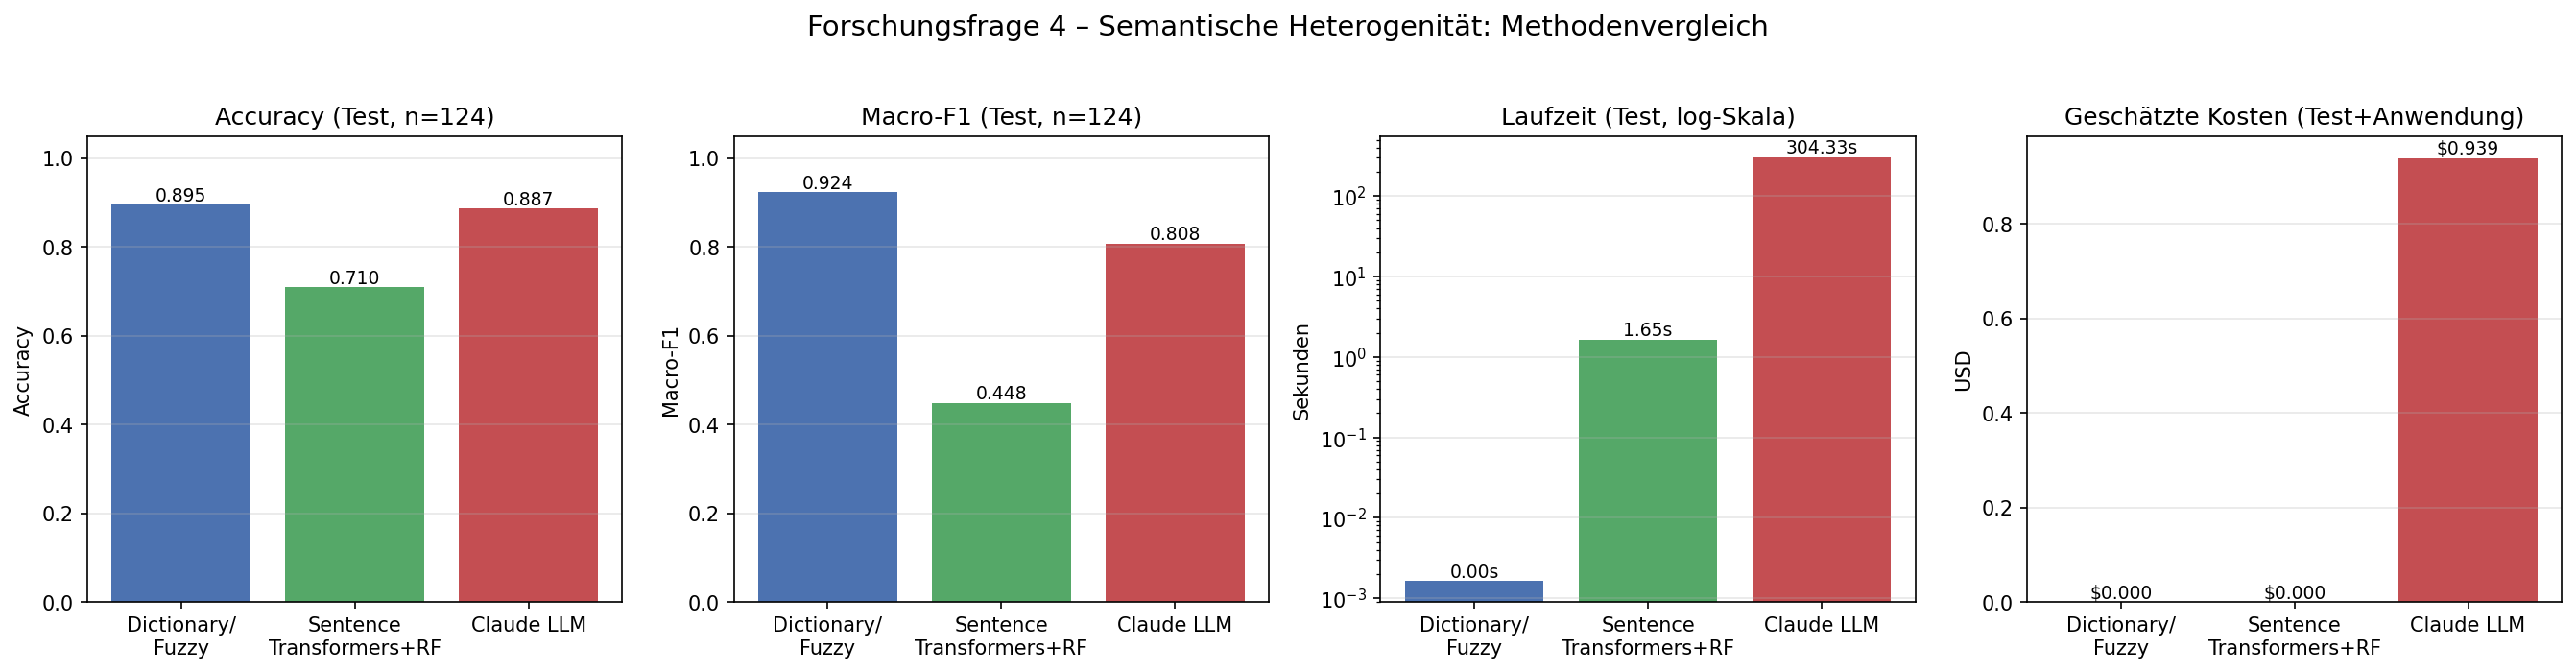
\includegraphics[width=0.85\textwidth]{images/tf4_methodenvergleich.png}
\caption{Methodenvergleich TF4 - Accuracy und Macro-F1 der semantischen Kategorienzuordnung}
\label{fig:tf4-methodenvergleich}
\end{figure}

Bemerkenswert ist, dass die einfachste Methode - eine aus dem Trainingssplit
gelernte Mehrheitszuordnungstabelle kombiniert mit Fuzzy-String-Matching als
Rückfallebene - hier sowohl das moderne Embedding-basierte Verfahren als auch
das LLM übertrifft. Dies erklärt sich aus der Struktur der Daten selbst: Die
Zuordnung von \texttt{thread\_category} zu \texttt{parent\_category} ist im
RedFlagDeals-Forum größtenteils redaktionell fest vorgegeben und damit nahezu
deterministisch, wodurch eine reine Nachschlagetabelle bereits einen Großteil
der Fälle korrekt löst.

\subsubsection{Der Grenzfall \enquote{Other}: Wenn semantisches Verständnis den entscheidenden Unterschied macht}

Alle 13 Fehlklassifikationen der Dictionary-Methode betreffen ausnahmslos
Fälle, in denen \texttt{thread\_category} den nichtssagenden Wert
\enquote{Other} trägt. Da \enquote{Other} im Trainingssplit am häufigsten mit
der \texttt{parent\_category} \enquote{Computers \& Electronics} assoziiert
ist, ordnet die Mehrheitstabelle \emph{jeden} \enquote{Other}-Fall dieser einen
Kategorie zu - unabhängig vom tatsächlichen Thema des jeweiligen Threads. In
der Praxis handelt es sich bei den 13 Fehlern jedoch überwiegend um Themen aus
den Bereichen \enquote{Home \& Garden} (7 von 13 Fällen), daneben
\enquote{Entertainment}, \enquote{Beauty \& Wellness}, \enquote{Kids \&
Babies}, \enquote{Automotive} und \enquote{Sports \& Fitness}. Das LLM, dem in
diesen Fällen (anders als der Dictionary-Methode) der vollständige Thread-Titel
zur semantischen Interpretation vorliegt, löst 6 dieser 13 \enquote{Other}-Grenzfälle
korrekt - etwa die richtige Zuordnung eines Automotive-Threads oder mehrerer
Home-\&-Garden-Threads -, scheitert jedoch ebenfalls an einigen mehrdeutigen
Fällen (z.\,B. wird ein \texttt{Kids \& Babies}-Thread fälschlich als
\texttt{Home \& Garden} eingeordnet). Dies zeigt exemplarisch die Grenze
tabellenbasierter Ansätze bei Threads ohne aussagekräftige granulare
Kategorie und den - hier nur teilweise realisierten - Mehrwert semantischen
Sprachverständnisses in genau diesen Randfällen.

\subsubsection{Warum das Embedding-Verfahren deutlich schlechter abschneidet}

Der auffällige Abstand zwischen Accuracy (0{,}710) und Macro-F1 (0{,}448) beim
Sentence-Transformers-Ansatz ist auf eine deutliche Klassen-Kollapstendenz
zurückzuführen: Von den 124 Testvorhersagen entfallen 73 (58,9\,\%) auf die
Klasse \enquote{Computers \& Electronics} und weitere 37 (29,8\,\%) auf
\enquote{Home \& Garden}, obwohl die wahre Verteilung deutlich breiter über
zwölf Kategorien gestreut ist (u.\,a. \enquote{Financial Services},
\enquote{Sports \& Fitness}, \enquote{Kids \& Babies}, \enquote{Travel} und
\enquote{Small Business}, die in den Vorhersagen des Modells \emph{kein
einziges Mal} auftauchen). Der auf 300-dimensionalen
\texttt{all-MiniLM-L6-v2}-Embeddings trainierte Random-Forest-Klassifikator
neigt bei der vorliegenden, kleinen und klassenunausgewogenen Trainingsmenge
offenbar dazu, seltene Kategorien systematisch zu ignorieren und stattdessen
auf die im Trainingssplit dominanten Klassen auszuweichen - ein klassisches
Symptom von Klassenungleichgewicht bei ressourcenarmem Training, das die
hohe (durch die dominanten Klassen getriebene) Accuracy verschleiert, aber im
klassengewichteten Macro-F1 deutlich sichtbar wird.

\subsubsection*{Zwischenfazit TF4}

TF4 liefert das methodisch vielleicht überraschendste Ergebnis dieser Arbeit:
Weder das moderne Embedding-Verfahren noch das LLM können die triviale,
aber datengetrieben parametrisierte Dictionary-Baseline schlagen, weil die
zugrunde liegende Zuordnungsstruktur der Daten selbst bereits stark
deterministisch ist. Gleichzeitig zeigt die detaillierte Analyse der
verbleibenden Grenzfälle (\enquote{Other}-Kategorie), dass echtes semantisches
Verständnis dort einen Mehrwert bietet, wo die granulare Ausgangsinformation
selbst uninformativ ist - ein Muster, das sich in abgeschwächter Form bereits
bei den Preis-Ausreißern in TF2 gezeigt hat.

% ---------------------------------------------------------------------
\subsection{Laufzeit-, Kosten- und Effizienzanalyse}
\label{sec:laufzeit-kosten}

Über alle vier Teilforschungsfragen hinweg wurden Laufzeit, Token-Verbrauch
und geschätzte API-Kosten für jede Methode protokolliert
(\texttt{results/laufzeit\_kosten\_log.csv}). Tabelle
\ref{tab:laufzeit-kosten} fasst die zentralen Kennzahlen zusammen.

\begin{table}[htbp]
\centering
\caption{Laufzeit und geschätzte Kosten je Methode und Teilaufgabe}
\label{tab:laufzeit-kosten}
\begin{tabularx}{\textwidth}{Xlrr}
\toprule
\rowcolor{headerblue}
\textbf{Teilaufgabe} & \textbf{Methode} & \textbf{Laufzeit (s)} & \textbf{Kosten (USD)} \\
\midrule
\rowcolor{lightgray}
TF1 Duplikate & RapidFuzz (Baseline) & 0{,}62 & 0{,}00 \\
TF1 Duplikate & Splink & 38{,}63 & 0{,}00 \\
\rowcolor{lightgray}
TF1 Duplikate & Claude LLM & 383{,}70 & 0{,}387 \\
TF2 price & Median (Baseline) & $<$0{,}01 & 0{,}00 \\
\rowcolor{lightgray}
TF2 price & RF n.\ MissForest-Prinzip & 1{,}53 & 0{,}00 \\
TF2 price & Claude LLM & 511{,}57 & 0{,}299 \\
\rowcolor{lightgray}
TF2 parent\_category & Modus (Baseline) & $<$0{,}01 & 0{,}00 \\
TF2 parent\_category & RF n.\ MissForest-Prinzip & 0{,}50 & 0{,}00 \\
\rowcolor{lightgray}
TF2 parent\_category & Claude LLM & 314{,}38 & 0{,}220 \\
TF3 price/saving/Datum & Regelbasiert & 0{,}12 & 0{,}00 \\
\rowcolor{lightgray}
TF3 price/saving & XGBoost-Parser & 0{,}33 & 0{,}00 \\
TF3 price/saving/Datum & Claude LLM & 2505{,}27 & 0{,}988 \\
\rowcolor{lightgray}
TF4 Semantik & Dictionary + Fuzzy & $<$0{,}01 & 0{,}00 \\
TF4 Semantik & Sentence-Transformers + RF & 1{,}65 & 0{,}00 \\
\rowcolor{lightgray}
TF4 Semantik & Claude LLM & 304{,}35 & 0{,}185 \\
\midrule
Finale Gesamtpipeline (1326 Zeilen) & Bester Methodenmix & \textbf{15{,}94} & \textbf{0{,}00} \\
\bottomrule
\end{tabularx}
\end{table}

Die Effizienzunterschiede sind über alle Experimente hinweg deutlich und
konsistent: Die klassischen und modernen Non-LLM-Methoden benötigen
durchgehend Bruchteile von Sekunden bis wenige Sekunden und verursachen keine
laufenden Kosten, während jede LLM-gestützte Verarbeitung mehrere Minuten in
Anspruch nimmt und messbare API-Kosten erzeugt. Über alle sieben
LLM-Teilaufgaben hinweg summieren sich die geschätzten Kosten dieser Arbeit
auf rund 2{,}08 USD bei einer Gesamtlaufzeit von ca. 67 Minuten - ein für
eine einmalige akademische Untersuchung dieser Größenordnung moderater
Betrag, der jedoch bei einer angenommenen Produktivanwendung auf den
vollständigen Datensatz (1326 statt im Schnitt rund 150-900 Testfällen je
Teilaufgabe) linear mit der Datenmenge skalieren würde und damit für
kontinuierliche, hochfrequente Datenbereinigungspipelines schnell
unwirtschaftlich werden kann. Die mit Abstand zeit- und kostenintensivste
Teilaufgabe ist die Datumsnormalisierung innerhalb von TF3 (Claude LLM:
1731{,}4 s bzw.\ 0{,}664 USD allein für diese eine Teilspalte), was primär auf
die hohe Fallzahl ($n = 885$) und die dabei anfallenden 217.144
Input-Tokens zurückzuführen ist - ein Bereich, in dem die
regelbasierte Regex-Kaskade bei \emph{identischer} Ergebnisqualität
(Exact-Match $= 1{,}0$ bei beiden Methoden) das LLM um mehr als das
15.000-fache in der Laufzeit unterbietet.

% ---------------------------------------------------------------------
\subsection{Anwendung der ausgewählten Methoden auf den Rohdatensatz}
\label{sec:finale-anwendung}

Auf Basis der in den Abschnitten \ref{sec:experiment-tf1} bis
\ref{sec:laufzeit-kosten} gewonnenen Erkenntnisse wurde abschließend eine
Gesamtpipeline aus den jeweils best geeigneten Methoden je Teilaufgabe
zusammengestellt und auf den vollständigen, unbereinigten Rohdatensatz
(1326 Zeilen) angewendet. Tabelle \ref{tab:finale-methodenwahl} dokumentiert
die getroffene Methodenwahl.

\begin{table}[htbp]
\centering
\caption{Finale Methodenwahl je Teilforschungsfrage für die Gesamtpipeline}
\label{tab:finale-methodenwahl}
\begin{tabular}{ll}
\toprule
\rowcolor{headerblue}
\textbf{Teilforschungsfrage} & \textbf{Gewählte Methode} \\
\midrule
\rowcolor{lightgray}
TF1 - Duplikate & Splink + regelbasierte Titel-Plausibilitätsprüfung \\
TF2 - Fehlende Werte (\texttt{price}) & Random Forest nach dem MissForest-Prinzip \\
\rowcolor{lightgray}
TF3 - Formatierung \texttt{price} & XGBoost-Parser \\
TF3 - Formatierung \texttt{saving} & Regelbasiert \\
\rowcolor{lightgray}
TF3 - Formatierung Datum & Regelbasiert \\
TF4 - Semantische Zuordnung & Dictionary + Fuzzy-Matching \\
\bottomrule
\end{tabular}
\end{table}

Diese Methodenwahl folgt konsequent dem in den vorangegangenen Abschnitten
etablierten Befund, dass moderne Non-LLM-Verfahren bei den meisten
Teilaufgaben eine mit dem LLM vergleichbare oder bei TF1/TF4 sogar leicht
überlegene Ergebnisqualität bei einem Bruchteil der Laufzeit und ohne
laufende API-Kosten liefern; einzig für die \texttt{price}-Imputation in TF2,
wo das LLM im direkten Methodenvergleich (Abschnitt \ref{sec:experiment-tf2})
den niedrigsten Fehler erzielte, wäre argumentierbar auch das LLM eine valide
Wahl gewesen - hier wurde jedoch aus Konsistenz- und Kostengründen ebenfalls
der moderne Non-LLM-Ansatz gewählt, da der Qualitätsunterschied
(MAE 176{,}34 vs. 154{,}30) vergleichsweise gering ausfällt.

\subsubsection{Ergebnis der Gesamtpipeline}

Tabelle \ref{tab:finale-ergebnisse} zeigt die zentralen Kennzahlen der
finalen Pipeline-Ausführung auf dem vollständigen Rohdatensatz.

\begin{table}[htbp]
\centering
\caption{Ergebnisse der finalen Gesamtpipeline auf dem vollständigen Rohdatensatz (1326 Zeilen)}
\label{tab:finale-ergebnisse}
\begin{tabular}{lr}
\toprule
\rowcolor{headerblue}
\textbf{Kennzahl} & \textbf{Wert} \\
\midrule
\rowcolor{lightgray}
Eingabezeilen & 1.326 \\
Erkannte und entfernte Duplikate & 20 \\
\rowcolor{lightgray}
Ausgabezeilen nach Bereinigung & 1.306 \\
Aufgefüllte fehlende \texttt{parent\_category}-Werte & 501 \\
\rowcolor{lightgray}
MAE \texttt{price} vs.\ Referenzdatensatz ($n{=}1052$) & 30{,}54 USD \\
MAE \texttt{saving} vs.\ Referenzdatensatz & $4{,}90 \times 10^{-5}$ \\
\rowcolor{lightgray}
Exact-Match \texttt{Datum} vs.\ Referenzdatensatz & 100\,\% \\
Gesamtlaufzeit der Pipeline & 15{,}94 s \\
\rowcolor{lightgray}
Gesamtkosten der Pipeline & 0{,}00 USD \\
\bottomrule
\end{tabular}
\end{table}

Von den ursprünglich 1326 Rohdatensatz-Zeilen wurden 20 als Duplikate
identifiziert und entfernt, sodass der finale bereinigte Datensatz 1306
eindeutige Einträge umfasst. Für 501 Zeilen, in denen
\texttt{parent\_category} fehlte, konnte die Dictionary-Methode einen Wert
ergänzen. Beim direkten Abgleich der price-Spalte mit dem unabhängigen
Referenzdatensatz (über das in Abschnitt 3.2.2 beschriebene inhaltsbasierte
Zeilen-Mapping, $n = 1052$ vergleichbare Zeilen) ergibt sich eine mittlere
absolute Abweichung von 30{,}54 USD - ein Wert, der angesichts der teils sehr
hohen absoluten Preisspannen im Datensatz (siehe Abschnitt 3.2.1) als gering
einzustufen ist. Die \texttt{saving}-Spalte stimmt mit dem Referenzdatensatz
nahezu perfekt überein (MAE $\approx 4{,}9 \times 10^{-5}$, praktisch
identisch mit einer exakten Übereinstimmung), und sämtliche normalisierten
Datumsangaben stimmen zu 100\,\% mit der Referenz überein. Bemerkenswert ist
zudem, dass sich die um ein Vielfaches höhere Datenmenge (1326 statt zuvor
im Schnitt 150-900 Testfälle je Einzelexperiment) durch die konsequente Wahl
schneller Non-LLM-Methoden in einer Gesamtlaufzeit von lediglich 15{,}94
Sekunden bei null laufenden API-Kosten niederschlägt - eine direkte
praktische Bestätigung des in Abschnitt \ref{sec:laufzeit-kosten}
diskutierten Effizienzvorteils, hochgerechnet auf den produktiven
Anwendungsfall.

\subsubsection*{Zwischenfazit: Anwendung auf den Rohdatensatz}

Die Übertragung der methodisch fundiert ausgewählten Non-LLM-dominierten
Pipeline auf den vollständigen Rohdatensatz bestätigt die in den
Einzelexperimenten gewonnenen Erkenntnisse auch im Maßstab des
Gesamtdatensatzes: Eine sorgfältig komponierte Kombination klassischer und
moderner Non-LLM-Verfahren erreicht eine gegenüber dem unabhängigen
Referenzdatensatz sehr hohe Übereinstimmung, bei einer für produktive
Anwendungen praxistauglichen Laufzeit von wenigen Sekunden und ohne laufende
Betriebskosten. Die in dieser Arbeit systematisch dokumentierten Grenzfälle
(Abschnitte \ref{sec:experiment-tf1} bis \ref{sec:experiment-tf4}) zeigen
jedoch auch, dass eine rein automatisierte Pipeline - unabhängig von der
gewählten Methodenklasse - niemals völlig fehlerfrei arbeitet und punktuelle
LLM-gestützte Nachprüfung insbesondere bei semantisch mehrdeutigen
Randfällen (z.\,B. der \enquote{Other}-Kategorie in TF4) einen gezielten,
kosteneffizient einsetzbaren Mehrwert bieten kann.
